
\section{일기도 그리기}

\subsection{지도 그리기}\index{지도 그리기}

Figure \ref{fig:mapofkorea01} \과 같은 지도를 그려보자.
\begin{figure}[h]
	\centering
	\includegraphics[width=0.7\linewidth]{MapOfKorea01}
	\caption{한반도 주변 지도(메르카토르도법)}
	\label{fig:mapofkorea01}
\end{figure}


\begin{code}[한반도 주변 지도(메르카토르도법)]
	\begin{lstlisting}
	
	#python 
	from mpl_toolkits.basemap import Basemap
	import matplotlib.pyplot as plt
	import numpy as np
	
	# create new figure, axes instances.
	fig = plt.figure()
	ax = fig.add_axes([0.1,0.1,0.8,0.8])
	
	#loglat = [west,south,east,north]
	loglat = [111,25,145,50]
	clog = (loglat[2]+loglat[0]) / 2
	clat = (loglat[3]+loglat[1]) / 2
	
	#map projection.
	m = Basemap(llcrnrlon=loglat[0],llcrnrlat=loglat[1],\
	urcrnrlon=loglat[2],urcrnrlat=loglat[3],\
	rsphere=(6378137.00,6356752.3142),\
	resolution='l',projection='merc',\
	lon_0=clog,lat_0=clat,lat_ts=20.)
	
	m.drawcoastlines()
	m.drawcountries()
	m.fillcontinents()
	
	# draw parallels
	m.drawparallels(np.arange(10,90,10),labels=[1,1,0,1])
	# draw meridians
	m.drawmeridians(np.arange(-180,180,10),labels=[1,1,0,1])
	
	plt.show()
	
	\end{lstlisting}
\end{code}

\subsection{일기도 모양의 지도 그리기}\index{일기도 모양의 지도 그리기}

Figure \ref{fig:surf201707021} \은 기상청(http://www.kma.go.kr/weather/images/analysischart.jsp)에서 제공하는 지상일기도이다. 

\begin{figure}[h]
	\centering
	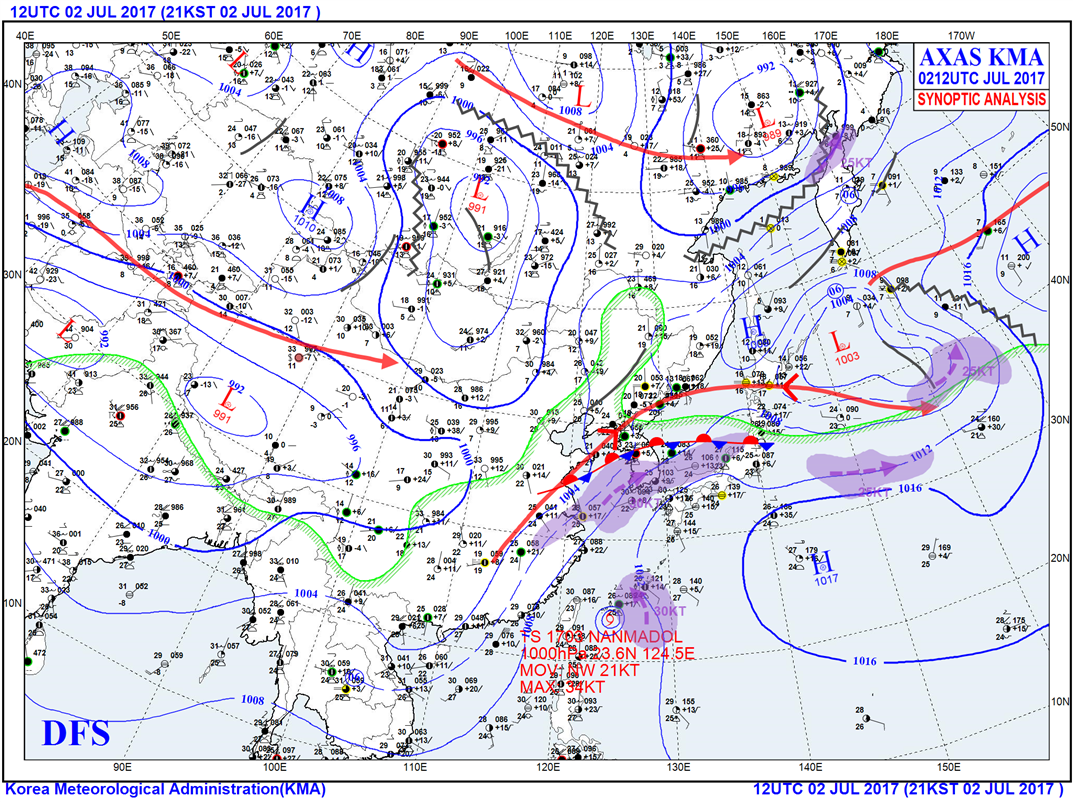
\includegraphics[width=0.8\linewidth]{surf_2017070212}
	\caption{기상청 지상일기도}
	\label{fig:surf2017070212}
\end{figure}

이와 비슷한 지도를 그리는 코드틑 다음과 같다.

\begin{code}[기상청 일기도모양 백지도]
	%	\begin{align}
	\begin{lstlisting}
	
	from mpl_toolkits.basemap import Basemap
	#python 
	import matplotlib.pyplot as plt
	import numpy as np
	
	# create new figure, axes instances.
	fig=plt.figure()
	ax=fig.add_axes([0.1,0.1,0.8,0.8])
	
	#loglat = [west,south,east,north]
	loglat = [90,0,180,62]
	clog = (loglat[2]+loglat[0])/2
	clat = (loglat[3]+loglat[1])/2
	
	# map projection.
	m = Basemap(llcrnrlon=loglat[0],llcrnrlat=loglat[1],\
	urcrnrlon=loglat[2],urcrnrlat=loglat[3],\
	resolution='l',projection='aea',lon_0=clog,lat_0=clat)
	
	m.drawcoastlines()
	m.drawcountries()
	m.fillcontinents()
	
	# draw parallels
	m.drawparallels(np.arange(0,90,10),labels=[1,1,0,0])
	# draw meridians
	m.drawmeridians(np.arange(-180,180,20),labels=[0,0,1,0])
	m.drawmeridians(np.arange(-180,180,10),labels=[0,0,0,1])
	
	plt.show()	
	\end{lstlisting}
	%		\end{align}
\end{code}

그 결과이다. 

\begin{figure}[h]
	\centering
	\includegraphics[width=0.8\linewidth]{weathermap01}
	\caption{기상청 일기도모양 백지도}
	\label{fig:weathermap01}
\end{figure}